\SourceLeaf{279}%
\Needspace{5\baselineskip}\begin{center}[2.]\end{center}

Der Beweis ist doch sehr leicht. Man nenne $n$ die Anzahl der Knoten
und bezeichne sie in der Folge, wie man sie trifft, indem man die
Curve in einem angenommenen Sinne der Bewegung durchläuft, durch
$1, 2, 3,\,.\,.\,.\,.\,n$. Da bei dieser Bewegung jeder Knoten zweimal getroffen
wird, so sei $\Omega$ die aus $2n$ Gliedern bestehende Reihe dieser Zahlen,
indem man das Zeichen $+$ beischreibt, so oft man auf die innere (rechte)
Seite des durchschnittenen Arms kommt, sonst $-$. Man zähle die $+$ und
$-$Zeichen bloss da zusammen, wo die Zahlen zum erstenmal vorkommen und
habe so $+\alpha$-, $-\beta$mal. Indem man nun die Charactere des Theils
der Curve, der zunächst vor dem ersten Knoten liegt, durch $\gamma,
\gamma'$ ausdrückt, ist die Amplitudo der ganzen Curve

\[
= (\gamma+\gamma'+\alpha-\beta)\,360^0.
\]

Es finden jedoch bei diesen Arrangements einige Bedingungen statt,
so dass nicht jedes aus der Luft gegriffene Arrangement möglich ist; jeder
Knoten muss einmal an einer geraden, einmal an einer ungeraden
Stelle vorkommen; zwischen den beiden Plätzen muss die Summe aller
$+\alpha, -\beta$ Null werden. Diess reicht aber nicht zu, um die
Unmöglichkeit des Schemas

\[
\begin{array}{@{}*{16}{c}@{}}
a&&b&&c&&b&&a&.&b&&c&&b&\\
&1&&2&&3&&1&&4&&3&&2&&4\\
&+&&-&&+&&-&&+&&-&&+&&-
\end{array}
\]

zu zeigen; hier müssen die Zeichen von 2 und 3 nothwendig geändert
werden\HistoricalNote{*)}{*)}{1844 Dec. 30 fand ich, dass die Anordnung der Zahlen (mittelste Reihe) \textls{zureicht}, um auch die zugehörigen Schnittcharactere ($+$ und $-$Zeichen in der untersten Reihe) und die Verknüpfung der Tracte (oberste Reihe) daraus abzuleiten, dass aber jene Anordnung selbst nicht willkürlich ist, sondern gewissen Bedingungen unterliegt, deren vollständige Ermittelung Gegenstand neuer Arbeiten sein wird. Es leidet jedoch auch der obige Satz Einschränkungen, z.\,B.
\begin{center}
\resizebox{2.6cm}{!}{%
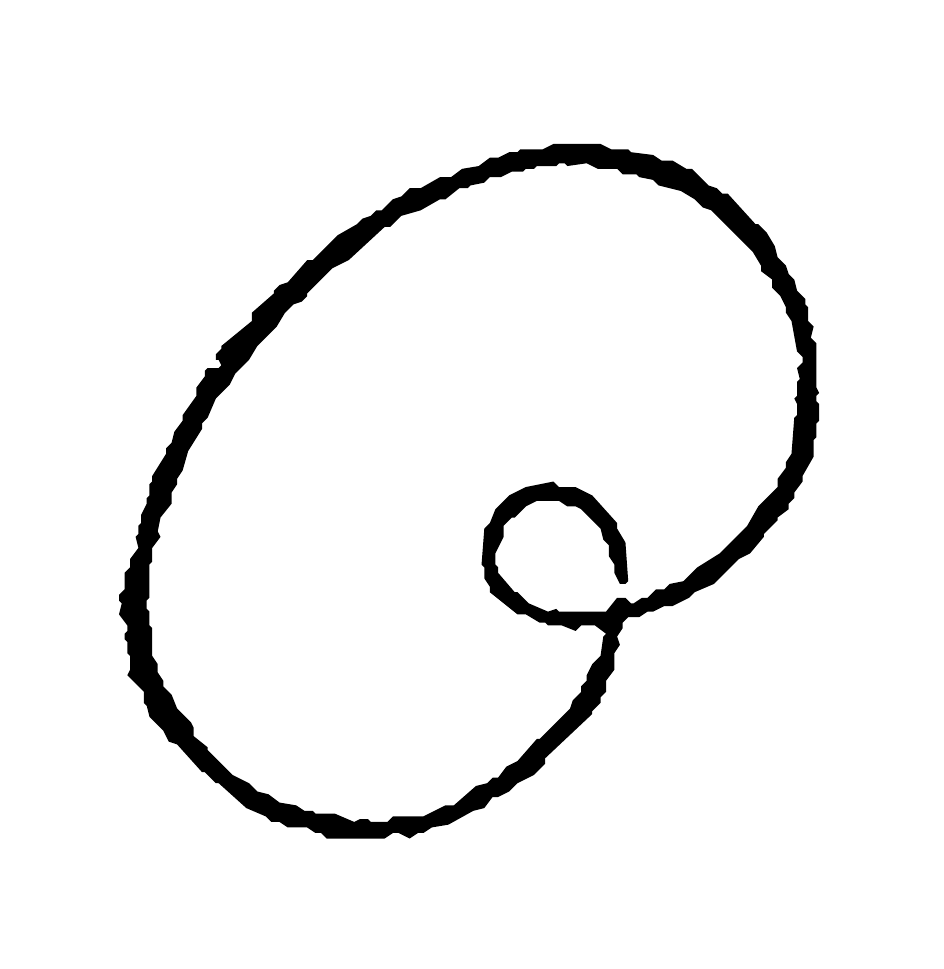
\begin{tikzpicture}[x=1pt,y=-1pt]
\path[use as bounding box] (0,0) rectangle (321,330);
\path[fill=black,draw=none,even odd rule]
(240,51) -- (238,51) -- (233,48) -- (229,48) -- (226,46) -- (218,45) -- (217,44) -- (211,44) -- (207,42) -- (190,42) -- (186,44) -- (178,44) -- (177,45) -- (174,45) -- (170,47) -- (167,47) -- (163,50) -- (157,51) -- (153,54) -- (149,54) -- (142,58) -- (138,58) -- (135,61) -- (132,62) -- (128,66) -- (126,66) -- (124,68) -- (121,69) -- (119,71) -- (112,75) -- (103,84) -- (101,84) -- (94,92) -- (91,93) -- (89,95) -- (89,96) -- (81,103) -- (81,106) -- (70,115) -- (70,116) -- (68,118) -- (68,120) -- (69,120) -- (70,122) -- (69,123) -- (65,123) -- (64,124) -- (64,126) -- (61,130) -- (61,133) -- (56,140) -- (56,142) -- (53,146) -- (52,150) -- (50,152) -- (50,154) -- (45,162) -- (45,164) -- (44,165) -- (44,169) -- (43,170) -- (43,172) -- (41,176) -- (41,179) -- (40,180) -- (40,183) -- (39,184) -- (40,188) -- (37,192) -- (37,195) -- (35,197) -- (35,203) -- (33,205) -- (33,207) -- (34,208) -- (33,212) -- (36,216) -- (36,218) -- (35,219) -- (35,221) -- (36,222) -- (36,226) -- (37,227) -- (37,232) -- (36,234) -- (42,240) -- (42,244) -- (43,245) -- (44,249) -- (49,254) -- (51,258) -- (54,259) -- (63,269) -- (64,269) -- (68,273) -- (69,273) -- (79,282) -- (86,285) -- (88,287) -- (91,287) -- (94,289) -- (101,289) -- (104,291) -- (106,291) -- (108,293) -- (129,293) -- (132,291) -- (134,291) -- (138,293) -- (141,291) -- (143,291) -- (146,289) -- (152,288) -- (161,283) -- (165,282) -- (168,278) -- (170,278) -- (174,276) -- (177,273) -- (183,270) -- (187,266) -- (187,264) -- (204,248) -- (204,247) -- (207,244) -- (207,242) -- (209,240) -- (209,236) -- (212,232) -- (212,226) -- (214,223) -- (213,220) -- (215,217) -- (215,215) -- (217,213) -- (221,213) -- (224,211) -- (226,211) -- (230,209) -- (233,209) -- (239,206) -- (241,204) -- (248,201) -- (257,192) -- (261,190) -- (266,184) -- (266,183) -- (271,178) -- (271,177) -- (275,174) -- (275,172) -- (277,170) -- (277,168) -- (280,164) -- (280,162) -- (284,155) -- (284,149) -- (285,148) -- (285,143) -- (286,142) -- (286,136) -- (285,135) -- (285,133) -- (286,132) -- (285,130) -- (285,114) -- (283,112) -- (284,108) -- (282,106) -- (282,101) -- (281,100) -- (281,98) -- (278,95) -- (277,91) -- (275,89) -- (274,86) -- (271,83) -- (270,79) -- (267,74) -- (264,71) -- (263,71) -- (253,60) -- (251,60) -- (249,58) -- (246,57) -- cycle
(247,66) -- (262,81) -- (265,86) -- (265,88) -- (269,91) -- (269,94) -- (272,97) -- (274,101) -- (274,103) -- (276,106) -- (278,117) -- (280,119) -- (280,121) -- (278,123) -- (279,127) -- (278,128) -- (278,133) -- (277,134) -- (278,136) -- (278,140) -- (277,141) -- (276,154) -- (274,157) -- (274,159) -- (271,163) -- (271,166) -- (264,173) -- (260,180) -- (250,190) -- (242,195) -- (237,200) -- (232,201) -- (230,203) -- (227,203) -- (224,206) -- (222,206) -- (219,208) -- (218,208) -- (216,206) -- (213,206) -- (209,211) -- (192,211) -- (191,210) -- (188,211) -- (181,208) -- (177,204) -- (176,204) -- (170,197) -- (170,195) -- (169,194) -- (169,190) -- (172,184) -- (172,180) -- (175,177) -- (176,177) -- (180,173) -- (184,171) -- (192,171) -- (195,173) -- (198,173) -- (200,174) -- (207,181) -- (208,185) -- (210,187) -- (210,191) -- (212,194) -- (212,197) -- (214,201) -- (216,201) -- (217,200) -- (216,186) -- (213,181) -- (213,179) -- (204,169) -- (198,166) -- (192,166) -- (190,164) -- (180,166) -- (174,169) -- (169,174) -- (167,179) -- (165,181) -- (164,194) -- (165,195) -- (165,199) -- (167,202) -- (167,204) -- (177,212) -- (180,212) -- (185,215) -- (187,215) -- (188,216) -- (193,216) -- (198,218) -- (200,216) -- (205,216) -- (209,219) -- (208,220) -- (207,227) -- (204,230) -- (202,234) -- (202,236) -- (200,238) -- (200,240) -- (197,243) -- (196,246) -- (185,257) -- (184,257) -- (177,265) -- (173,267) -- (170,271) -- (168,271) -- (166,273) -- (162,274) -- (154,281) -- (151,281) -- (143,285) -- (132,285) -- (130,287) -- (124,287) -- (123,286) -- (120,286) -- (118,287) -- (111,284) -- (104,284) -- (103,283) -- (100,283) -- (97,281) -- (91,280) -- (87,277) -- (83,276) -- (80,273) -- (74,270) -- (65,261) -- (65,260) -- (60,256) -- (60,253) -- (59,251) -- (54,246) -- (52,241) -- (49,238) -- (49,236) -- (47,233) -- (47,230) -- (45,227) -- (45,217) -- (44,216) -- (44,211) -- (43,210) -- (43,207) -- (44,206) -- (44,194) -- (45,193) -- (45,188) -- (48,184) -- (47,182) -- (48,177) -- (52,172) -- (52,168) -- (54,165) -- (54,163) -- (56,160) -- (58,153) -- (63,145) -- (63,143) -- (65,141) -- (68,134) -- (73,129) -- (75,125) -- (80,120) -- (83,115) -- (90,108) -- (93,103) -- (96,100) -- (99,99) -- (101,97) -- (101,96) -- (110,87) -- (116,84) -- (129,72) -- (131,72) -- (135,68) -- (142,66) -- (149,62) -- (151,62) -- (156,58) -- (159,58) -- (160,57) -- (165,56) -- (167,54) -- (171,54) -- (175,52) -- (179,52) -- (180,51) -- (183,51) -- (184,50) -- (191,50) -- (192,49) -- (194,49) -- (195,50) -- (202,49) -- (206,51) -- (213,51) -- (215,53) -- (220,53) -- (221,54) -- (226,55) -- (228,57) -- (236,59) -- (241,62) -- (244,65) -- cycle;
\end{tikzpicture}%
}
\hfill
\resizebox{3.4cm}{!}{%
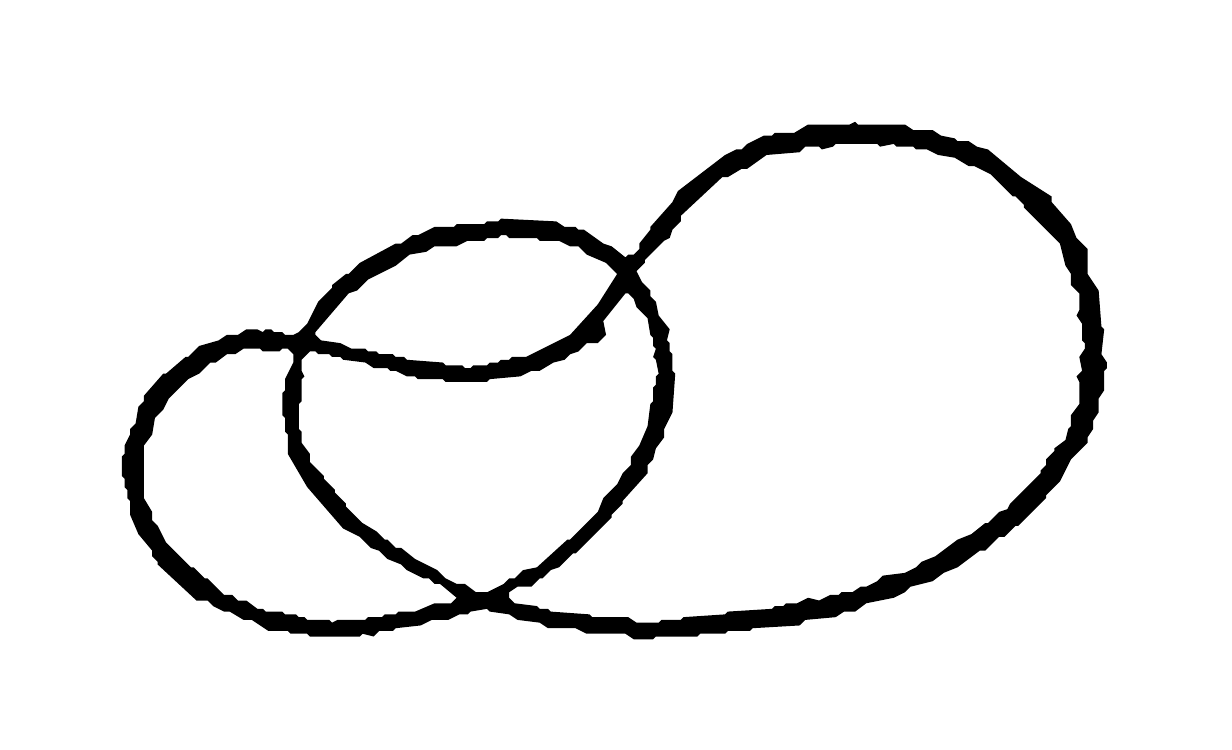
\begin{tikzpicture}[x=1pt,y=-1pt]
\path[use as bounding box] (0,0) rectangle (425,251);
\path[fill=black,draw=none,even odd rule]
(383,80) -- (379,76) -- (377,71) -- (370,63) -- (370,61) -- (359,54) -- (347,44) -- (343,43) -- (340,41) -- (336,41) -- (335,40) -- (330,39) -- (327,37) -- (320,37) -- (317,35) -- (300,35) -- (299,34) -- (297,35) -- (282,35) -- (277,38) -- (270,38) -- (269,39) -- (266,39) -- (260,42) -- (258,44) -- (256,44) -- (252,46) -- (235,59) -- (233,63) -- (225,72) -- (225,73) -- (221,78) -- (221,80) -- (219,82) -- (217,82) -- (216,83) -- (211,79) -- (208,78) -- (201,73) -- (199,73) -- (198,72) -- (194,72) -- (191,70) -- (171,69) -- (170,70) -- (166,70) -- (165,71) -- (155,71) -- (154,72) -- (147,72) -- (141,75) -- (139,75) -- (135,78) -- (133,78) -- (120,85) -- (116,89) -- (115,89) -- (110,93) -- (110,94) -- (105,99) -- (101,107) -- (98,110) -- (96,111) -- (93,111) -- (92,110) -- (89,110) -- (88,109) -- (86,109) -- (85,110) -- (83,109) -- (79,109) -- (76,111) -- (72,111) -- (69,113) -- (62,115) -- (58,119) -- (57,119) -- (50,125) -- (49,125) -- (42,133) -- (42,135) -- (40,137) -- (39,143) -- (37,145) -- (37,147) -- (35,151) -- (35,154) -- (34,155) -- (34,162) -- (35,163) -- (35,166) -- (36,167) -- (36,170) -- (37,171) -- (37,176) -- (40,183) -- (45,189) -- (45,191) -- (47,193) -- (47,194) -- (61,207) -- (65,207) -- (67,209) -- (71,211) -- (73,211) -- (78,214) -- (81,214) -- (87,218) -- (94,218) -- (95,219) -- (101,219) -- (102,220) -- (120,220) -- (121,219) -- (125,220) -- (127,218) -- (132,218) -- (133,217) -- (142,216) -- (146,214) -- (152,214) -- (156,212) -- (159,212) -- (160,211) -- (166,210) -- (167,211) -- (174,212) -- (177,214) -- (185,215) -- (188,217) -- (198,217) -- (202,219) -- (216,219) -- (219,221) -- (226,221) -- (227,220) -- (242,220) -- (243,219) -- (252,219) -- (253,218) -- (261,218) -- (262,217) -- (279,216) -- (281,214) -- (292,213) -- (295,211) -- (299,211) -- (303,208) -- (313,206) -- (317,204) -- (319,202) -- (327,200) -- (331,197) -- (336,195) -- (344,189) -- (346,189) -- (351,184) -- (353,184) -- (357,180) -- (358,180) -- (368,170) -- (368,169) -- (373,164) -- (377,156) -- (383,150) -- (383,148) -- (385,145) -- (385,142) -- (387,139) -- (387,134) -- (389,131) -- (389,124) -- (390,123) -- (390,121) -- (388,118) -- (389,109) -- (388,108) -- (387,95) -- (383,89) -- cycle
(46,141) -- (49,138) -- (51,134) -- (58,127) -- (62,125) -- (66,121) -- (68,121) -- (72,118) -- (75,118) -- (78,116) -- (84,116) -- (85,117) -- (91,117) -- (92,116) -- (94,116) -- (96,118) -- (96,121) -- (93,127) -- (93,131) -- (92,132) -- (92,140) -- (93,141) -- (93,146) -- (94,147) -- (94,154) -- (101,166) -- (114,181) -- (120,184) -- (124,188) -- (127,189) -- (130,192) -- (135,194) -- (137,196) -- (143,199) -- (145,199) -- (147,201) -- (149,201) -- (155,206) -- (153,208) -- (147,208) -- (140,211) -- (134,211) -- (133,212) -- (129,212) -- (128,213) -- (123,213) -- (122,214) -- (112,214) -- (110,215) -- (109,214) -- (101,214) -- (100,213) -- (98,213) -- (97,212) -- (93,212) -- (92,211) -- (86,211) -- (85,210) -- (83,210) -- (79,207) -- (76,207) -- (74,205) -- (71,205) -- (65,199) -- (64,199) -- (60,195) -- (59,195) -- (50,186) -- (47,180) -- (45,178) -- (45,175) -- (42,170) -- (42,151) -- (45,147) -- cycle
(224,105) -- (225,111) -- (226,112) -- (226,115) -- (227,116) -- (226,119) -- (227,120) -- (228,125) -- (227,126) -- (227,129) -- (226,130) -- (226,135) -- (225,136) -- (224,144) -- (221,151) -- (218,155) -- (218,158) -- (215,161) -- (213,165) -- (208,170) -- (206,175) -- (196,185) -- (195,185) -- (184,195) -- (179,196) -- (176,199) -- (174,199) -- (172,201) -- (166,204) -- (162,204) -- (158,201) -- (155,201) -- (151,199) -- (148,196) -- (140,192) -- (135,188) -- (133,188) -- (130,185) -- (129,185) -- (126,182) -- (121,179) -- (115,173) -- (115,172) -- (111,168) -- (111,167) -- (107,163) -- (107,162) -- (102,157) -- (102,154) -- (99,150) -- (99,146) -- (98,145) -- (98,136) -- (99,135) -- (99,127) -- (100,126) -- (99,124) -- (99,120) -- (102,117) -- (104,117) -- (105,118) -- (109,118) -- (110,119) -- (113,119) -- (114,120) -- (122,121) -- (125,123) -- (130,123) -- (131,124) -- (133,124) -- (137,126) -- (140,126) -- (141,127) -- (150,127) -- (151,128) -- (166,128) -- (167,127) -- (178,126) -- (182,124) -- (185,124) -- (190,121) -- (194,120) -- (196,118) -- (199,117) -- (202,114) -- (206,114) -- (209,111) -- (208,106) -- (216,96) -- (217,96) -- (219,98) -- (220,101) -- cycle
(213,89) -- (206,100) -- (196,111) -- (180,119) -- (175,119) -- (174,120) -- (171,120) -- (170,121) -- (167,121) -- (166,122) -- (161,122) -- (160,123) -- (158,123) -- (157,122) -- (151,122) -- (150,121) -- (137,120) -- (136,119) -- (133,119) -- (132,118) -- (127,118) -- (126,117) -- (123,117) -- (122,116) -- (117,116) -- (113,114) -- (106,113) -- (104,111) -- (104,110) -- (116,96) -- (119,95) -- (123,91) -- (133,86) -- (138,82) -- (144,81) -- (147,79) -- (155,79) -- (159,77) -- (165,77) -- (166,76) -- (170,76) -- (171,75) -- (173,75) -- (174,76) -- (184,76) -- (185,77) -- (192,77) -- (196,79) -- (199,79) -- (202,82) -- (209,85) -- cycle
(373,78) -- (375,86) -- (377,89) -- (377,93) -- (380,96) -- (380,102) -- (379,104) -- (381,107) -- (381,113) -- (382,114) -- (382,116) -- (380,119) -- (381,124) -- (379,126) -- (380,128) -- (380,136) -- (377,140) -- (377,144) -- (376,145) -- (375,149) -- (371,152) -- (371,153) -- (368,156) -- (368,158) -- (366,160) -- (366,161) -- (355,172) -- (354,174) -- (351,175) -- (347,179) -- (346,179) -- (341,183) -- (336,185) -- (328,191) -- (323,193) -- (321,195) -- (317,197) -- (309,198) -- (307,200) -- (303,202) -- (301,202) -- (298,204) -- (294,204) -- (293,205) -- (290,205) -- (286,207) -- (282,206) -- (278,208) -- (274,208) -- (273,209) -- (270,209) -- (269,210) -- (253,211) -- (252,212) -- (237,213) -- (236,214) -- (229,214) -- (228,215) -- (220,215) -- (217,213) -- (204,213) -- (203,212) -- (189,211) -- (188,210) -- (185,210) -- (184,209) -- (176,208) -- (174,206) -- (174,204) -- (177,202) -- (182,202) -- (185,199) -- (186,199) -- (189,196) -- (192,195) -- (197,190) -- (198,190) -- (211,177) -- (211,176) -- (215,172) -- (215,171) -- (224,161) -- (224,158) -- (226,156) -- (227,152) -- (230,148) -- (230,145) -- (233,139) -- (234,125) -- (233,124) -- (233,118) -- (232,117) -- (232,114) -- (231,113) -- (232,109) -- (228,104) -- (227,99) -- (225,97) -- (225,95) -- (222,92) -- (220,88) -- (223,85) -- (223,84) -- (230,77) -- (232,76) -- (233,73) -- (236,70) -- (236,68) -- (251,54) -- (253,54) -- (258,51) -- (260,51) -- (267,46) -- (279,45) -- (281,43) -- (286,43) -- (287,44) -- (291,43) -- (292,42) -- (307,42) -- (308,43) -- (313,42) -- (314,43) -- (320,43) -- (321,44) -- (325,44) -- (329,46) -- (335,47) -- (340,50) -- (342,50) -- (348,53) -- (356,61) -- (357,61) -- (360,64) -- (360,65) -- cycle;
\end{tikzpicture}%
}
\hfill
\resizebox{4.4cm}{!}{%
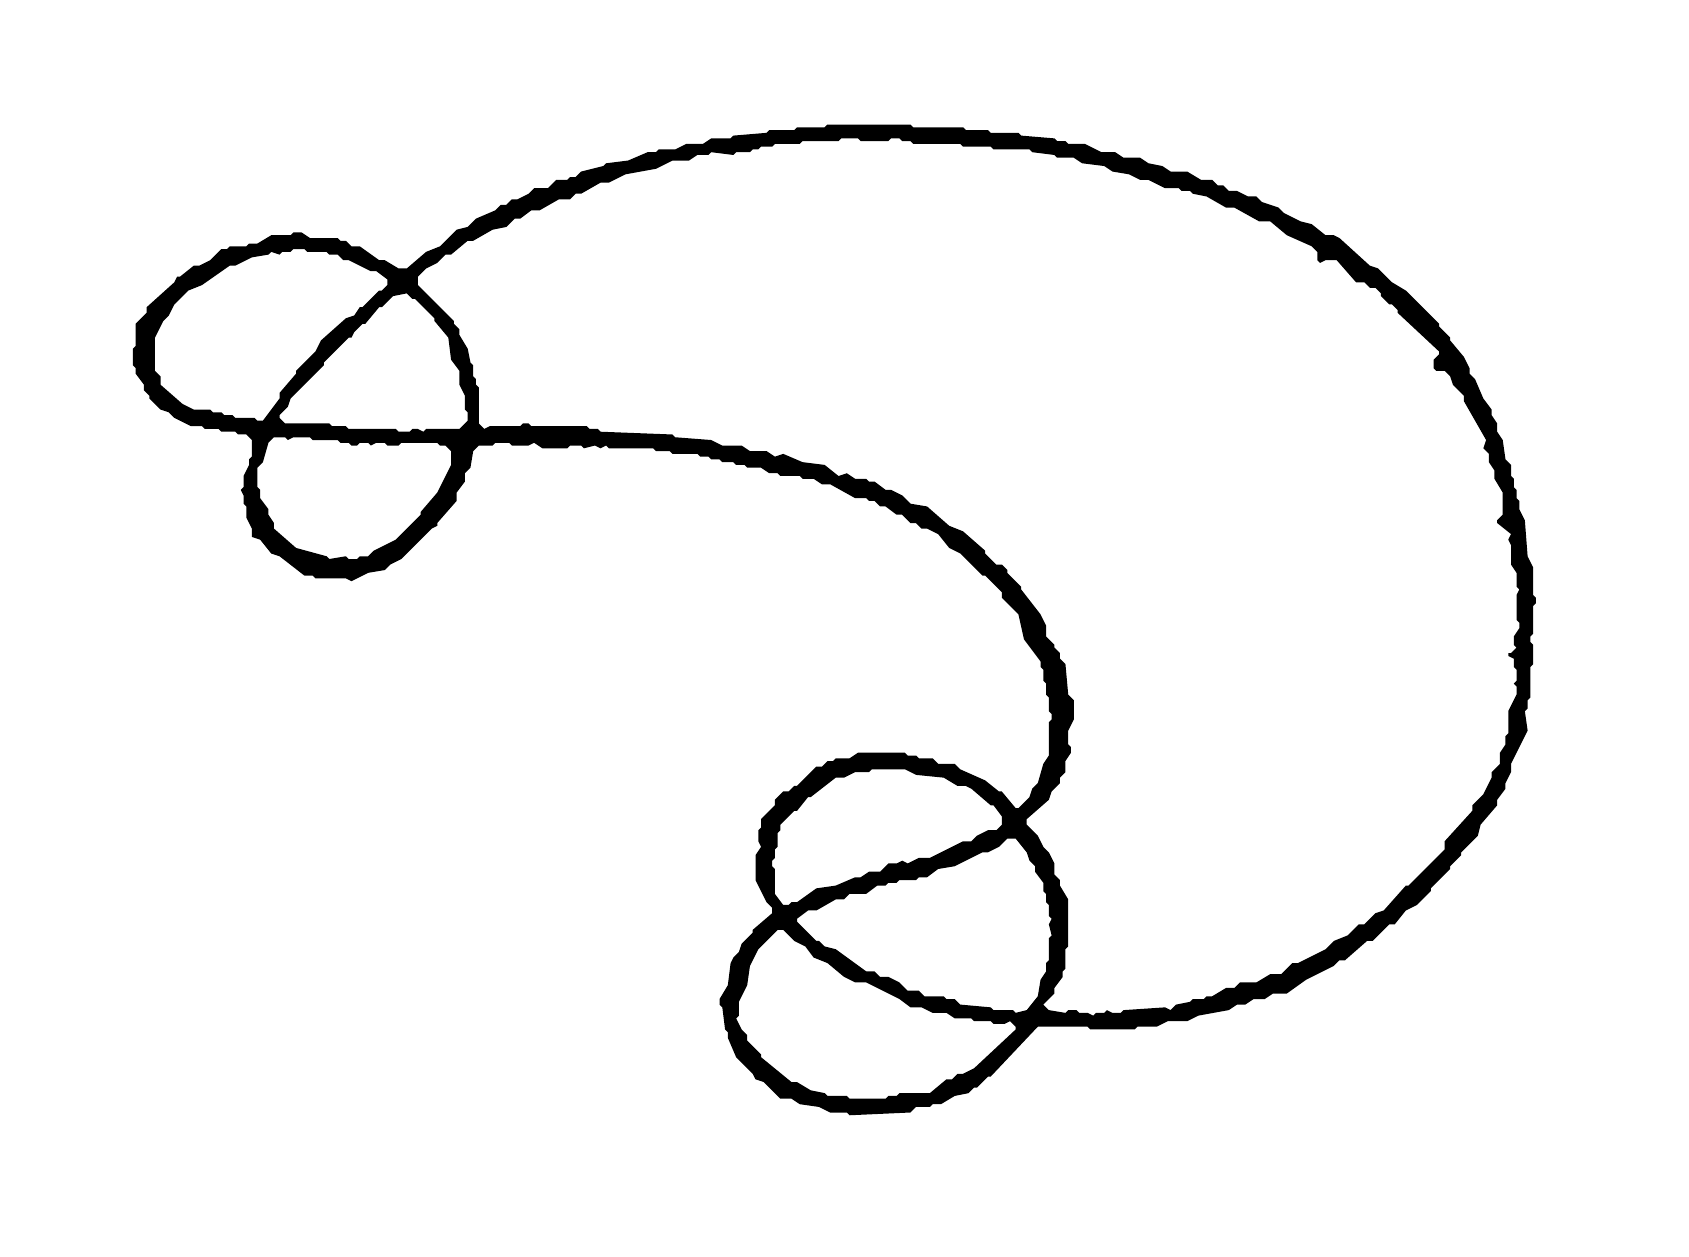
\begin{tikzpicture}[x=1pt,y=-1pt]
\path[use as bounding box] (0,0) rectangle (590,434);
\path[fill=black,draw=none,even odd rule]
(54,90) -- (53,92) -- (43,101) -- (43,103) -- (39,107) -- (39,115) -- (38,116) -- (38,122) -- (39,123) -- (39,125) -- (42,129) -- (42,131) -- (44,133) -- (44,134) -- (48,138) -- (51,139) -- (53,141) -- (59,144) -- (63,144) -- (64,145) -- (69,145) -- (70,146) -- (75,146) -- (76,147) -- (79,147) -- (81,149) -- (81,155) -- (80,156) -- (80,158) -- (78,162) -- (78,166) -- (77,167) -- (78,169) -- (78,172) -- (79,173) -- (79,177) -- (81,181) -- (81,184) -- (84,185) -- (88,190) -- (91,191) -- (100,198) -- (103,198) -- (104,199) -- (115,199) -- (117,200) -- (123,197) -- (129,196) -- (131,194) -- (135,192) -- (146,181) -- (148,180) -- (148,179) -- (155,171) -- (155,168) -- (158,164) -- (158,161) -- (160,159) -- (161,153) -- (163,151) -- (168,151) -- (169,150) -- (174,150) -- (175,151) -- (181,151) -- (183,150) -- (186,152) -- (195,152) -- (196,151) -- (200,151) -- (201,152) -- (205,151) -- (207,152) -- (209,151) -- (210,152) -- (226,152) -- (227,153) -- (232,153) -- (233,154) -- (242,154) -- (243,155) -- (246,155) -- (247,156) -- (250,156) -- (251,157) -- (255,157) -- (256,158) -- (259,158) -- (260,159) -- (265,159) -- (268,161) -- (271,161) -- (272,162) -- (279,162) -- (280,163) -- (284,163) -- (287,165) -- (290,165) -- (299,170) -- (303,170) -- (304,171) -- (306,171) -- (308,173) -- (310,173) -- (314,176) -- (316,176) -- (319,179) -- (321,179) -- (323,181) -- (325,181) -- (329,183) -- (333,188) -- (337,190) -- (345,198) -- (346,198) -- (352,204) -- (352,206) -- (358,212) -- (360,221) -- (366,229) -- (366,231) -- (367,232) -- (367,236) -- (368,237) -- (368,241) -- (369,242) -- (369,247) -- (370,248) -- (370,250) -- (369,251) -- (369,263) -- (367,266) -- (365,273) -- (363,275) -- (362,278) -- (358,282) -- (357,282) -- (352,276) -- (351,276) -- (346,272) -- (337,268) -- (335,266) -- (329,266) -- (327,264) -- (322,264) -- (321,263) -- (318,263) -- (317,262) -- (300,262) -- (297,264) -- (292,264) -- (291,265) -- (289,265) -- (287,267) -- (285,267) -- (278,274) -- (277,274) -- (275,276) -- (273,276) -- (270,279) -- (270,281) -- (265,286) -- (265,289) -- (264,290) -- (264,294) -- (265,296) -- (263,299) -- (263,308) -- (267,316) -- (269,318) -- (269,320) -- (262,326) -- (262,327) -- (258,331) -- (257,334) -- (255,336) -- (254,338) -- (253,346) -- (250,351) -- (250,353) -- (251,354) -- (252,362) -- (253,363) -- (253,365) -- (256,372) -- (262,378) -- (263,380) -- (266,381) -- (272,387) -- (276,387) -- (279,389) -- (286,390) -- (290,392) -- (296,392) -- (297,393) -- (319,392) -- (321,390) -- (326,390) -- (327,389) -- (330,389) -- (335,386) -- (340,385) -- (342,383) -- (343,383) -- (347,379) -- (348,379) -- (365,361) -- (383,361) -- (384,362) -- (400,362) -- (401,361) -- (408,361) -- (412,359) -- (419,359) -- (423,357) -- (434,355) -- (437,353) -- (440,353) -- (443,351) -- (447,351) -- (450,349) -- (455,349) -- (462,344) -- (472,339) -- (474,337) -- (476,337) -- (484,330) -- (486,330) -- (492,324) -- (494,324) -- (498,319) -- (502,317) -- (507,312) -- (507,311) -- (514,304) -- (514,303) -- (518,299) -- (518,298) -- (524,292) -- (525,288) -- (531,281) -- (531,279) -- (534,275) -- (534,273) -- (536,269) -- (536,266) -- (542,254) -- (541,247) -- (542,246) -- (542,243) -- (543,242) -- (543,231) -- (544,230) -- (544,223) -- (543,222) -- (543,220) -- (544,219) -- (544,209) -- (545,208) -- (545,206) -- (544,205) -- (544,195) -- (542,191) -- (541,178) -- (539,174) -- (539,171) -- (538,170) -- (538,167) -- (537,166) -- (537,163) -- (536,162) -- (536,158) -- (534,156) -- (533,149) -- (531,146) -- (531,143) -- (529,140) -- (529,138) -- (526,134) -- (523,127) -- (521,125) -- (521,123) -- (519,119) -- (514,113) -- (514,112) -- (510,108) -- (510,107) -- (498,95) -- (493,92) -- (488,87) -- (485,86) -- (474,76) -- (472,75) -- (469,75) -- (464,71) -- (460,70) -- (454,67) -- (452,65) -- (446,63) -- (444,61) -- (441,61) -- (437,59) -- (434,59) -- (432,57) -- (430,57) -- (428,55) -- (424,55) -- (419,52) -- (413,52) -- (410,50) -- (405,49) -- (402,47) -- (396,47) -- (393,45) -- (388,45) -- (382,42) -- (376,42) -- (375,41) -- (372,41) -- (371,40) -- (359,39) -- (358,38) -- (348,38) -- (347,37) -- (339,37) -- (338,36) -- (320,36) -- (319,35) -- (289,35) -- (288,36) -- (278,36) -- (277,37) -- (268,37) -- (267,38) -- (255,39) -- (254,40) -- (247,40) -- (244,42) -- (238,42) -- (234,44) -- (228,44) -- (227,45) -- (224,45) -- (217,48) -- (209,49) -- (208,50) -- (200,52) -- (198,54) -- (196,54) -- (195,55) -- (191,55) -- (188,58) -- (183,58) -- (181,60) -- (177,62) -- (175,62) -- (173,64) -- (171,64) -- (169,66) -- (162,69) -- (159,72) -- (155,73) -- (149,79) -- (144,81) -- (137,87) -- (134,87) -- (129,84) -- (127,84) -- (120,79) -- (117,79) -- (115,77) -- (113,77) -- (112,76) -- (102,76) -- (99,74) -- (96,74) -- (95,75) -- (88,75) -- (83,78) -- (80,78) -- (79,79) -- (73,79) -- (72,80) -- (70,80) -- (66,84) -- (62,86) -- (60,86) -- (55,90) -- cycle
(256,358) -- (257,357) -- (257,352) -- (260,346) -- (261,339) -- (264,333) -- (271,326) -- (273,326) -- (277,330) -- (281,332) -- (284,336) -- (289,338) -- (295,343) -- (299,345) -- (303,345) -- (315,351) -- (319,354) -- (323,354) -- (327,356) -- (332,356) -- (335,358) -- (341,358) -- (342,359) -- (348,359) -- (349,360) -- (353,360) -- (355,359) -- (357,361) -- (357,362) -- (342,376) -- (338,378) -- (336,378) -- (334,380) -- (332,380) -- (326,385) -- (315,385) -- (314,386) -- (311,386) -- (310,387) -- (297,387) -- (296,386) -- (289,386) -- (288,385) -- (283,384) -- (278,381) -- (276,381) -- (265,372) -- (265,371) -- (260,366) -- (260,364) -- (258,362) -- cycle
(370,328) -- (369,329) -- (369,337) -- (368,338) -- (368,341) -- (366,344) -- (365,350) -- (361,355) -- (357,356) -- (356,355) -- (349,355) -- (348,354) -- (337,353) -- (335,351) -- (332,351) -- (331,350) -- (324,350) -- (322,348) -- (318,348) -- (315,345) -- (311,343) -- (308,343) -- (306,341) -- (303,341) -- (292,333) -- (288,332) -- (286,330) -- (285,330) -- (278,323) -- (278,322) -- (282,319) -- (285,319) -- (292,315) -- (295,315) -- (297,313) -- (303,313) -- (307,310) -- (310,310) -- (311,309) -- (314,309) -- (315,308) -- (321,308) -- (322,307) -- (325,307) -- (329,304) -- (335,303) -- (345,298) -- (347,298) -- (351,296) -- (354,293) -- (357,293) -- (361,298) -- (362,301) -- (364,303) -- (364,305) -- (367,309) -- (367,312) -- (368,313) -- (368,316) -- (369,317) -- (369,321) -- (370,322) -- (369,324) -- cycle
(352,285) -- (352,288) -- (350,290) -- (347,290) -- (343,292) -- (341,294) -- (338,294) -- (326,300) -- (322,300) -- (318,302) -- (316,301) -- (314,302) -- (311,302) -- (308,305) -- (304,305) -- (301,307) -- (299,307) -- (292,310) -- (285,311) -- (278,316) -- (276,316) -- (275,317) -- (273,317) -- (270,313) -- (270,304) -- (269,303) -- (269,301) -- (270,300) -- (270,297) -- (271,296) -- (271,291) -- (272,290) -- (272,288) -- (277,283) -- (278,283) -- (282,278) -- (283,278) -- (292,271) -- (295,271) -- (299,269) -- (304,269) -- (305,268) -- (317,268) -- (321,270) -- (331,271) -- (336,274) -- (339,274) -- (341,275) -- (348,281) -- (349,281) -- cycle
(83,166) -- (83,159) -- (85,157) -- (87,150) -- (89,148) -- (93,148) -- (94,149) -- (96,148) -- (102,148) -- (103,149) -- (112,149) -- (113,150) -- (116,150) -- (117,151) -- (119,151) -- (120,150) -- (123,150) -- (124,151) -- (126,150) -- (129,150) -- (130,151) -- (134,151) -- (135,150) -- (148,150) -- (149,151) -- (151,151) -- (153,153) -- (153,158) -- (148,168) -- (142,175) -- (142,176) -- (133,185) -- (125,189) -- (123,191) -- (120,191) -- (119,192) -- (116,192) -- (115,191) -- (109,192) -- (108,191) -- (97,188) -- (89,181) -- (89,179) -- (87,176) -- (87,174) -- (84,170) -- (84,167) -- cycle
(152,112) -- (153,120) -- (156,124) -- (156,129) -- (158,133) -- (158,138) -- (159,139) -- (159,142) -- (156,145) -- (144,145) -- (143,146) -- (141,145) -- (139,145) -- (138,146) -- (134,146) -- (133,145) -- (116,145) -- (115,144) -- (110,144) -- (109,143) -- (93,143) -- (91,141) -- (91,140) -- (94,137) -- (95,134) -- (107,122) -- (107,121) -- (116,112) -- (117,112) -- (118,110) -- (121,107) -- (122,107) -- (127,101) -- (128,101) -- (132,97) -- (137,96) -- (139,98) -- (140,98) -- (147,105) -- (147,106) -- cycle
(130,91) -- (130,93) -- (128,95) -- (127,95) -- (121,101) -- (120,101) -- (118,104) -- (115,105) -- (106,113) -- (104,117) -- (97,124) -- (97,125) -- (91,132) -- (91,134) -- (85,142) -- (83,142) -- (82,141) -- (75,141) -- (74,140) -- (71,140) -- (70,139) -- (67,139) -- (66,138) -- (60,138) -- (56,136) -- (48,129) -- (48,126) -- (46,124) -- (46,112) -- (49,106) -- (51,104) -- (53,100) -- (58,95) -- (63,93) -- (73,86) -- (75,86) -- (81,83) -- (87,82) -- (88,81) -- (91,82) -- (92,81) -- (95,81) -- (96,80) -- (100,80) -- (101,81) -- (108,81) -- (109,82) -- (112,82) -- (114,84) -- (116,84) -- (124,88) -- (126,88) -- cycle
(141,90) -- (144,87) -- (148,85) -- (151,82) -- (153,82) -- (159,77) -- (161,77) -- (168,73) -- (173,72) -- (176,69) -- (178,69) -- (182,66) -- (185,66) -- (192,62) -- (196,62) -- (198,60) -- (200,60) -- (207,56) -- (210,56) -- (216,53) -- (227,51) -- (233,48) -- (239,48) -- (242,46) -- (246,46) -- (247,45) -- (255,46) -- (256,45) -- (261,45) -- (262,44) -- (264,44) -- (265,43) -- (269,43) -- (270,42) -- (279,42) -- (280,41) -- (293,41) -- (294,40) -- (300,40) -- (301,41) -- (311,41) -- (312,40) -- (315,40) -- (316,41) -- (319,41) -- (320,42) -- (337,42) -- (338,43) -- (348,43) -- (349,44) -- (362,44) -- (363,45) -- (371,46) -- (372,47) -- (378,47) -- (381,49) -- (389,50) -- (392,52) -- (398,53) -- (402,55) -- (405,55) -- (411,58) -- (416,58) -- (417,59) -- (420,59) -- (421,60) -- (426,61) -- (433,65) -- (436,65) -- (445,70) -- (449,70) -- (455,75) -- (464,79) -- (466,81) -- (466,84) -- (467,85) -- (469,84) -- (473,84) -- (480,92) -- (483,92) -- (485,94) -- (487,94) -- (489,96) -- (489,97) -- (492,100) -- (493,100) -- (495,102) -- (495,103) -- (510,117) -- (510,118) -- (508,120) -- (508,123) -- (509,124) -- (512,124) -- (514,126) -- (515,129) -- (519,133) -- (519,135) -- (527,149) -- (526,152) -- (528,154) -- (528,157) -- (530,160) -- (530,163) -- (533,168) -- (533,176) -- (531,178) -- (531,179) -- (536,183) -- (535,185) -- (536,187) -- (536,194) -- (538,197) -- (538,202) -- (539,203) -- (538,205) -- (538,214) -- (539,215) -- (539,217) -- (537,220) -- (537,223) -- (538,224) -- (536,226) -- (535,226) -- (535,227) -- (537,228) -- (537,231) -- (538,232) -- (538,236) -- (537,237) -- (538,238) -- (538,241) -- (535,247) -- (535,255) -- (534,256) -- (534,259) -- (532,262) -- (532,266) -- (529,269) -- (529,271) -- (526,277) -- (522,281) -- (522,283) -- (512,294) -- (512,297) -- (499,310) -- (498,310) -- (490,319) -- (487,320) -- (483,324) -- (481,324) -- (477,328) -- (472,330) -- (469,333) -- (459,338) -- (457,338) -- (453,342) -- (449,342) -- (444,345) -- (438,345) -- (436,347) -- (433,347) -- (428,350) -- (426,350) -- (425,351) -- (421,351) -- (420,352) -- (415,353) -- (413,355) -- (411,354) -- (396,355) -- (395,356) -- (392,356) -- (390,355) -- (389,356) -- (386,356) -- (385,357) -- (383,356) -- (380,356) -- (379,355) -- (376,355) -- (375,356) -- (369,355) -- (367,353) -- (371,349) -- (371,347) -- (374,343) -- (374,341) -- (375,340) -- (375,333) -- (376,332) -- (376,315) -- (373,310) -- (373,308) -- (371,306) -- (371,302) -- (369,298) -- (367,296) -- (365,292) -- (361,288) -- (361,286) -- (369,279) -- (370,276) -- (373,273) -- (373,271) -- (375,269) -- (375,265) -- (377,262) -- (377,260) -- (376,259) -- (376,254) -- (378,250) -- (378,243) -- (376,241) -- (375,230) -- (373,228) -- (373,226) -- (371,224) -- (371,223) -- (368,220) -- (368,216) -- (366,212) -- (359,203) -- (359,202) -- (354,197) -- (354,196) -- (352,194) -- (350,194) -- (346,190) -- (346,189) -- (338,182) -- (333,180) -- (325,173) -- (319,172) -- (316,169) -- (312,167) -- (310,167) -- (306,164) -- (304,164) -- (303,163) -- (299,163) -- (296,161) -- (293,162) -- (288,158) -- (280,157) -- (273,154) -- (270,155) -- (267,153) -- (261,153) -- (258,151) -- (251,151) -- (247,149) -- (234,148) -- (233,147) -- (207,146) -- (206,145) -- (203,145) -- (202,144) -- (182,144) -- (181,143) -- (179,143) -- (178,144) -- (167,144) -- (165,145) -- (163,143) -- (163,130) -- (162,129) -- (162,127) -- (161,126) -- (161,122) -- (160,121) -- (159,116) -- (156,111) -- (156,109) -- (154,107) -- (154,106) -- (141,93) -- cycle;
\end{tikzpicture}%
}

\end{center}
}.

